\section{Modellbasierte Darstellung des Geschäftsprozesses}\label{sec:bpmnabbildung}
Durch die fachlich sowie technisch konzipierten Anwendungsfall der Fertigungsdurchführung ergibt sich das, in Abbildung \ref{fig:Darstellung der dynamischen Fertigungsdurchführung} dargestellte, Geschäftsprozessmodell. 

Es zeichnet sich im besonderen Maße durch eine ausgeprägte Orientierung an den relevanten Ereignissen der Fertigungsdurchführung aus. Durch die dynamische Wechselwirkung zwischen den Aktivitäten und Ereignissen wird es möglich gemacht in Echtzeit Anpassungen am Geschäftsprozess durchzuführen. Des Weiteren werden unnötige Aktivitäten der ursprünglichen Fertigungsdurchführung durch digitale Dienste ersetzt. Duch die automatisierte Benachrichtigung des Werkers  über neue Fertigungsaufträge und Plausibilitätsprüfungen zur Laufzeit können Latenzen, die durch überflüssige Laufwege enstehen maßgeblich reduziert werden.

Des Weiteren werden grundlegende Aspekte des Lean Management wie die Erfassung von Defekten in den Geschäftsprozess integriert. Dies soll die Fähigkeit in Echtzeit auf kritische Ereignisse zu reagieren, durch eine verbesserte Transparenz der Problemstellen, um ein Vielfaches steigern.

\begin{figure}[H]
	\centering 
	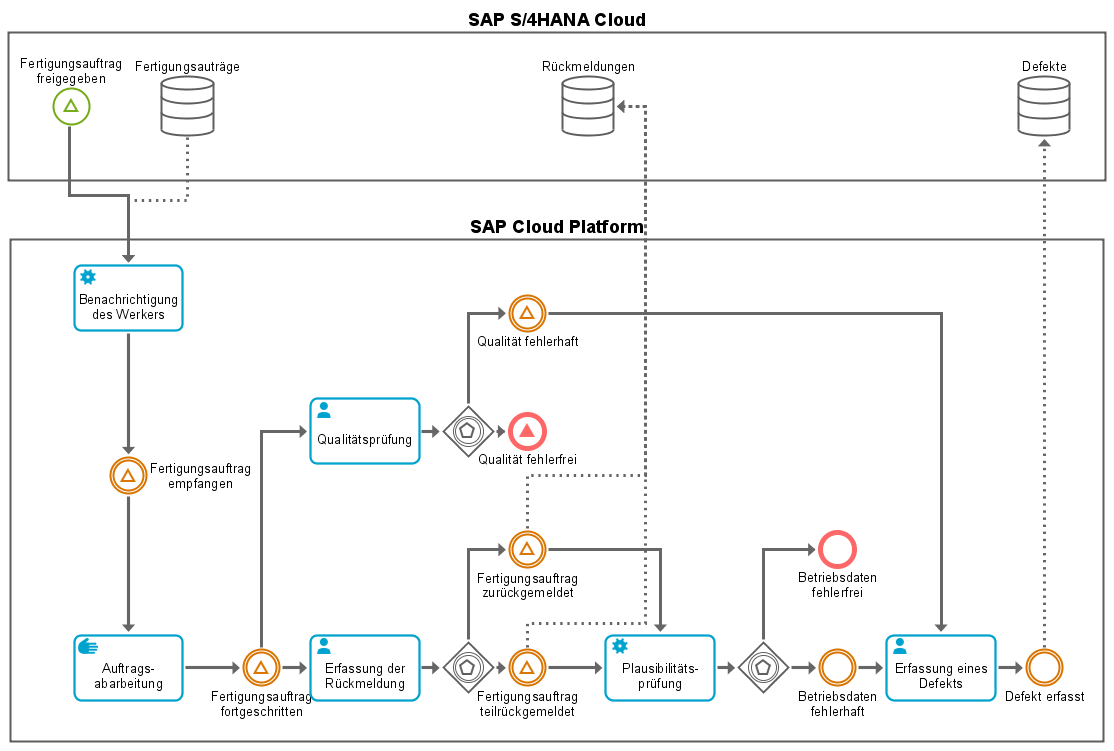
\includegraphics[width=1.4\textwidth, angle =90 ]{img/gesamt.png}
	\caption[Darstellung der dynamischen Fertigungsdurchführung]{\label{fig:Darstellung der dynamischen Fertigungsdurchführung}Darstellung der dynamischen Fertigungsdurchführung
	}
\end{figure}